\chapter{Theorie}
\section{Das Spiel Tic-Tac-Toe}

Tic-Tac-Toe ist ein sehr altes, klassisches Strategiespiel, welches von zwei Personen gespielt wird. Eine Person
spielt hierbei das Symbol Kreuz und eine andere Person das Symbol Kreis. Das Spielfeld von Tic-Tac-Toe besteht aus
neun Feldern, in denen die entsprechenden Symbole verteilt werden können. Jeder Spieler setzt hierzu abwechselnd sein
Symbol in eines der neun Felder. Es ist nicht möglich ein bestehendes Symbol zu überschreiben oder mehrere Symbole in
ein Feld zu zeichnen. Der Anfang einer Runde Tic-Tac-Toe kann beispielsweise wie folgt aussehen:
\begin{figure}[H]
    \centering
    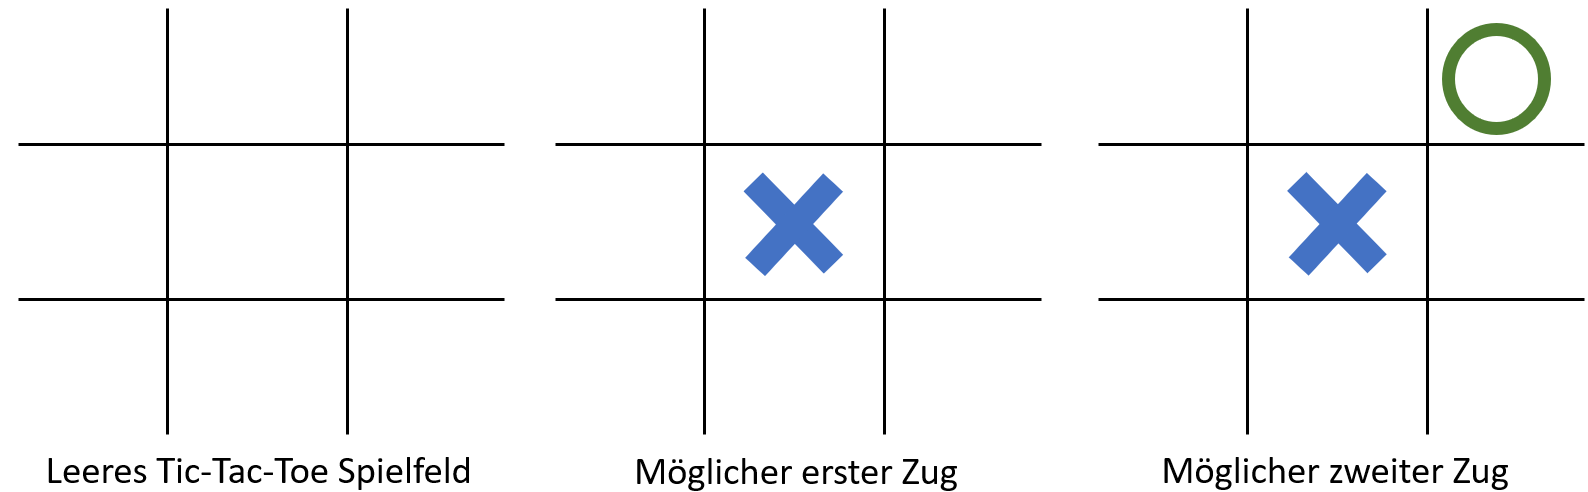
\includegraphics[scale=0.25]{img/tictactoe_start.png}
    \caption[Möglicher Anfang eines Tic-Tac-Toe Spiels]{Möglicher Anfang eines Tic-Tac-Toe Spiels (eigene Anfertigung)}
\end{figure}
Im ersten Teil des Bildes erkennt man die neun leeren Felder des Spielfeldes. Im zweiten Teil des Bildes fängt der erste
Spieler damit an, sein erstes Kreuz in die Mitte des Spielfeldes zu setzen. Der zweite Spieler ist nun am Zug und setzt
im dritten Teil des Bildes seinen Kreis in die obere rechte Ecke des Spielfeldes. Als nächstes wäre Spieler eins wieder an
der Reihe und dürfte sein nächstes Kreuz setzen. Ziel des Spiels ist es, drei gleiche Symbole in einer Reihe, Spalte oder
Diagonale zu haben. Die folgende Abbildung soll dieses Verfahren nochmal genauer erläutern:
\begin{figure}[H]
    \centering
    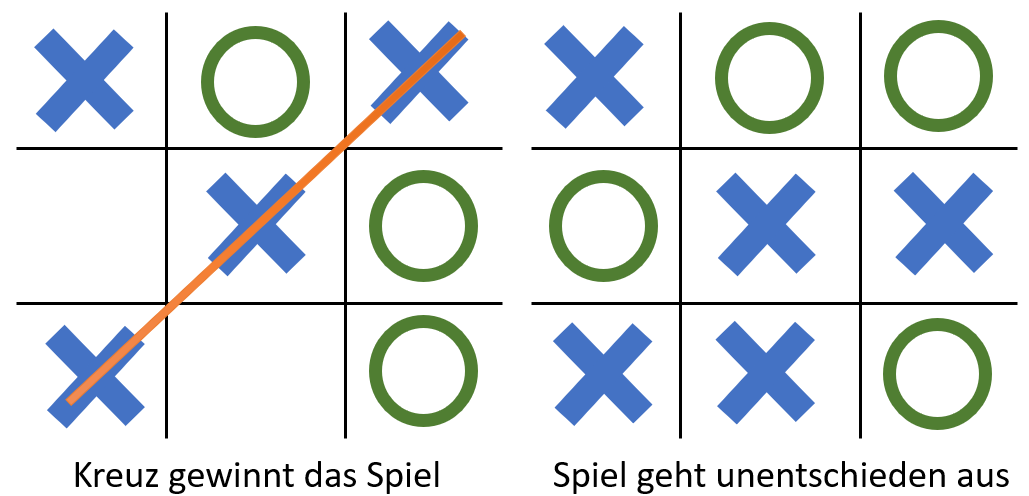
\includegraphics[scale=0.25]{img/tictactoe_endings.png} 
    \caption[Mögliches Ende eines Tic-Tac-Toe Spiels]{Mögliches Ende eines Tic-Tac-Toe Spiels (eigene Anfertigung)}
\end{figure}
Im ersten Teil der Abbildung ist zu sehen, wie der Spieler mit dem Kreuzsymbol drei Kreuze auf einer Diagonale unterbringen
konnte. In diesem Fall ist die Runde beendet und dieser Spieler hat die Runde gewonnen. Ob das Spiel über drei Symbole in einer
Reihe, Spalte oder Diagonale gewonnen wird, ist nicht relevant. Ebenfalls spielt es keine Rolle, in welcher Reihenfolge die 
Symbole gesetzt wurden. Im zweiten Teil des Bildes zeigt sich ein weiteres mögliches Ende für eine Runde Tic-Tac-Toe. Bei diesem
Ende ist das komplette Spielfeld ausgefüllt und es ergeben sich keine drei Symbole in einer Reihe, Spalte oder Diagonale. 
Entsprechend ist die Runde unentschieden ausgegangen.

\section{Der Minimax-Algorithmus}
Nachdem das Spiel Tic-Tac-Toe erklärt wurde, soll nun mit Hilfe des Minimax Algorithmus eine künstliche Intelligenz 
entwickelt werden, die in einem Spiel gegen einen menschlichen Spieler immer einen optimalen Zug ausführt. Der Minimax 
Algorithmus baut dabei auf der Funktion \code{value} auf, die wie folgt definiert ist:

\[value: States \times Players \rightarrow \{-1,0,1\}\]

Die Rückgabewert symbolisieren dabei den worst case Ausgang eines Zuges:

\begin{itemize}
    \item -1 bedeutet, dass der Spieler bei diesem Spielzug im schlechtesten Fall verliert
    \item 0 bedeutet, dass im schlechtesten Fall ein Unentschieden erzielt werden kann
    \item 1 bedeutet, dass mit der Wahl dieses Spielzuges ein Sieg erzielt wird
\end{itemize}

Die Funktion berechnet alle möglichen Folgezüge für das übergebene Spielfeld. Sobald eine Spielsituation 
erreicht wurde, bei der das Spiel entweder von einem Spieler gewonnen wurde oder keine weiteren Spielsteine 
mehr gesetzt werden können, wird die Funktion \code{utility} aufgerufen. Diese vergleicht den Spielzustand 
mit allen möglichen Endzuständen und gibt gegebenenfall den Gewinner oder Unentschieden zurück. Da der Spieler 
nach jedem Zug wechselt wird immer abwechselnd der höchste Wert bzw. der niedrigste Wert für den nächsten Zug gewählt.

Betrachten wir dies an einem Beispiel:
\begin{figure}[H]
    \centering
    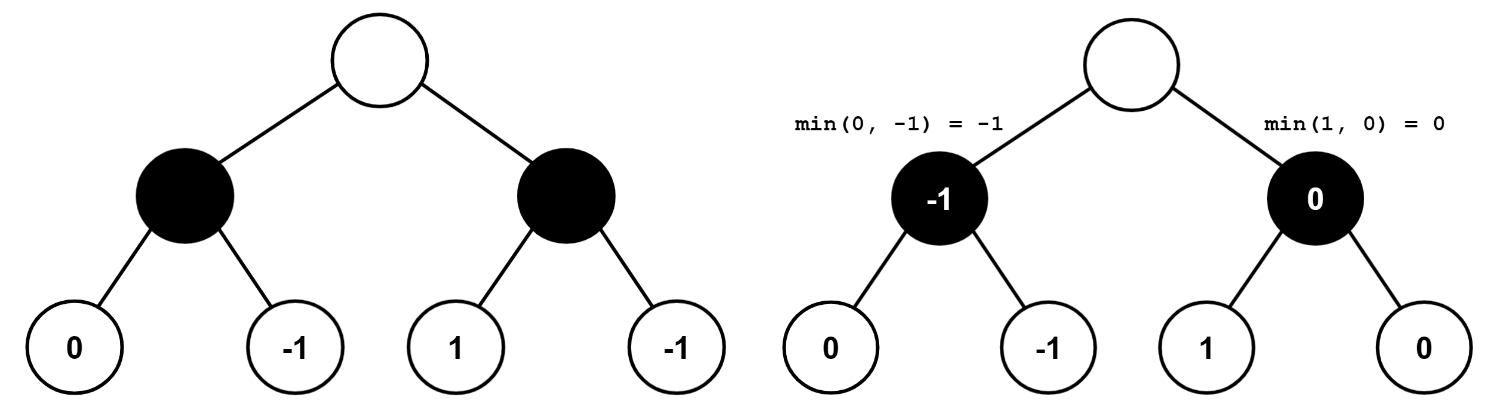
\includegraphics[scale=0.4]{img/minimax_step_0.png}
    \caption[Beispiel für die Auswahl eines Zuges mit dem Minimax-Algorithmus]{Beispiel für die Auswahl eines Zuges mit dem Minimax-Algorithmus \\ (eigene Anfertigung)}
\end{figure}

In diesem Fall gibt es zwei mögliche nächste Züge. Wichtig ist, dass nach jedem Zug der Spieler wechselt und der Algorithmus 
immer davon ausgehen muss, dass der Gegner den Zug mit dem höchsten Wert für ihn, also dem niedrigsten Wert für die KI wählt. 
Für das Beispiel heißt das, dass wenn der Gegner am Zug ist (schwarze Knoten), er den niedrigsten Wert, hier also -1 wählt. 
Das gleiche gilt für den zweiten schwarzen Knoten, wo der Wert 0 ausgewählt wird.

Im nächsten Schritt ist die KI wieder am Zug, also wird diesmal der maximale Wert der möglichen Züge bestimmt. Konkret heißt das, 
dass wenn der rechte Zug gewählt wird, im schlechtesten Fall ein Unentschieden und beim linken Zug eine Niederlage erzielt werden kann. 
Um die Niederlage abzuwenden wird der rechte Zug und damit der höhere Wert gewählt.

\begin{figure}[H]
    \centering
    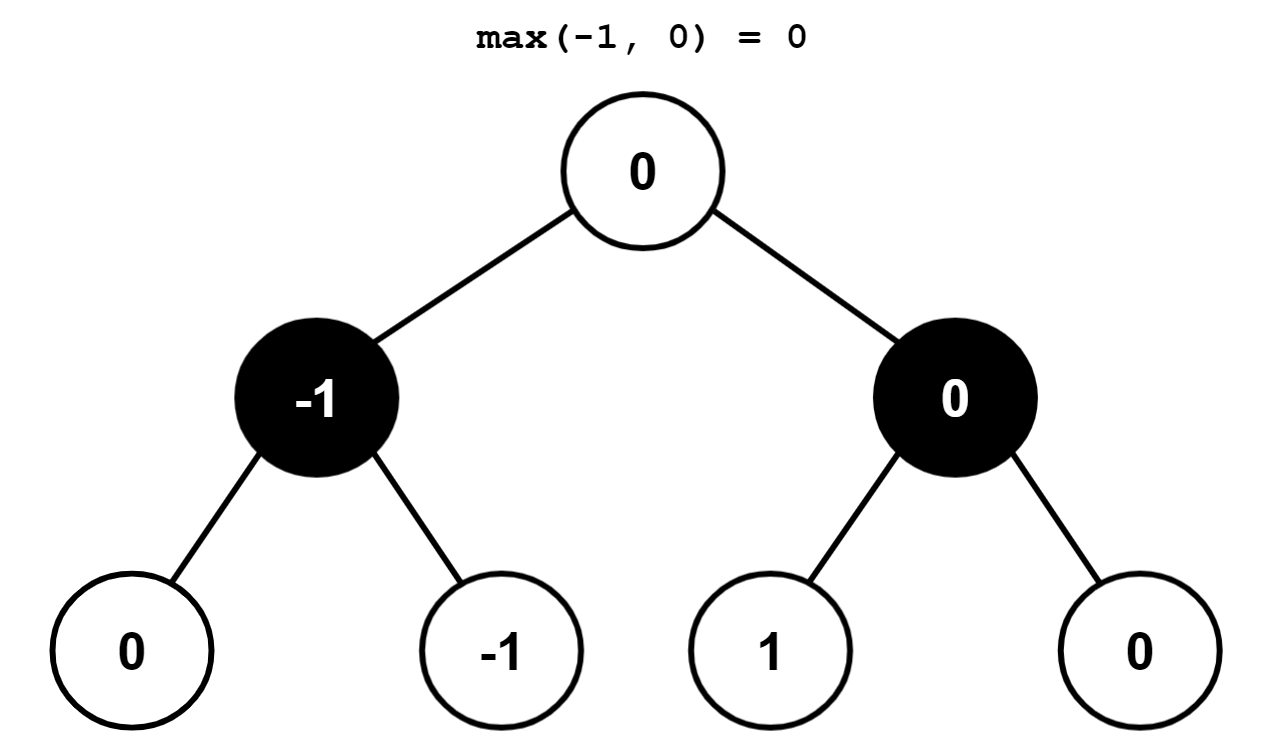
\includegraphics[scale=0.25]{img/minimax_step_1.png}
    \caption[Auswahl des finalen Spielzuges]{Auswahl des finalen Spielzuges (eigene Anfertigung)}
\end{figure}

Anzumerken ist, dass bei jedem Aufruf der Funktion \code{value} alle weiteren möglichen Spielzüge berechnet werden. 
Beim Spiel Tic-Tac-Toe kann es vorkommen, dass mehrere unterschiedliche Spielverläufe im selben Zustand enden. 
Für die Funktion \code{value} heißt das, dass sie mehrfach mit den selben Parametern aufgerufen wird und dadurch 
Rechenleistung verschwendet wird. Um redundante Funktionsaufrufe zu vermeiden wird das Prinzip der Memoisierung 
verwendet. D. h. es wird z. B. ein Dictionary verwendet, um bereits berechnete Ergebnisse zu speichern. Wird nun 
die Funktion \code{value} aufgerufen, wird erst geprüft, ob für die Parameter bereits ein Eintrag im Dictionary 
vorhanden ist. Ist dies der Fall wird dieser Wert zurückgegeben und es findet keine Berechnung statt. Ist dem nicht 
so, wird ein neuer Eintrag im Dictionary angelegt.